% IEEE SMC 2026 style figures (PGFPlots + TikZ)

\begin{figure}[t]
\centering
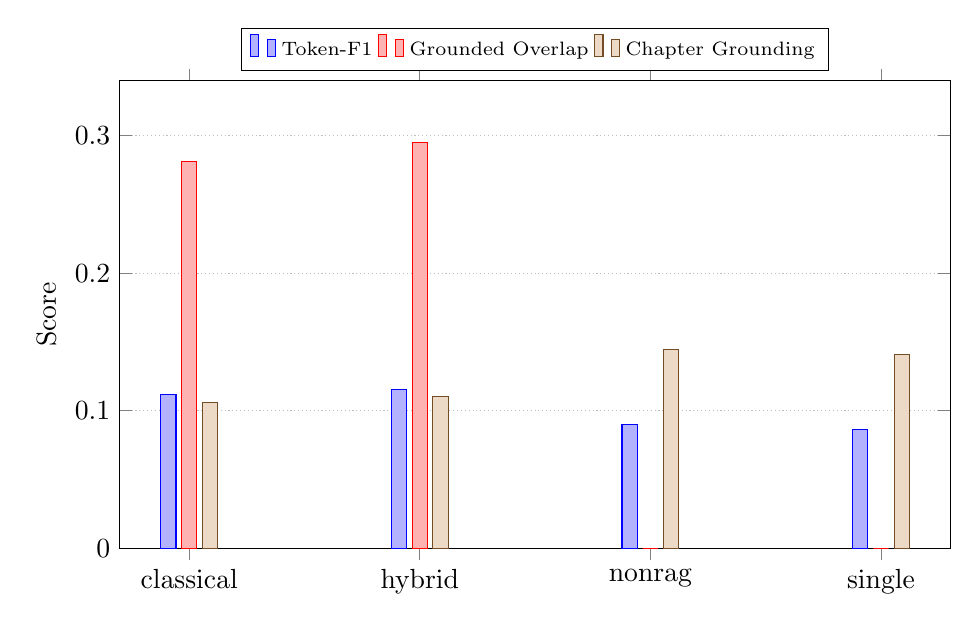
\begin{tikzpicture}
\begin{axis}[
    width=\columnwidth,
    height=0.62\columnwidth,
    ybar,
    bar width=5.5pt,
    ymin=0,
    ymax=0.34,
    symbolic x coords={classical,hybrid,nonrag,single},
    xtick=data,
    ylabel={Score},
    legend style={font=\scriptsize, at={(0.5,1.02)}, anchor=south, legend columns=3},
    ymajorgrids=true,
    grid style=densely dotted
]
\addplot coordinates {(classical,0.1115) (hybrid,0.1152) (nonrag,0.0898) (single,0.0865)};
\addplot coordinates {(classical,0.2812) (hybrid,0.2953) (nonrag,0.0000) (single,0.0000)};
\addplot coordinates {(classical,0.1057) (hybrid,0.1101) (nonrag,0.1445) (single,0.1411)};
\legend{Token-F1,Grounded Overlap,Chapter Grounding}
\end{axis}
\end{tikzpicture}
\caption{TutorEval lexical and grounding metrics. Hybrid Fast dominates token-level and retrieval-grounded overlap, while chapter grounding peaks in non-RAG settings because this metric can also fire via chapter-context overlap.}
\label{fig:tutoreval_grounding_profile}
\end{figure}

\begin{figure}[t]
\centering
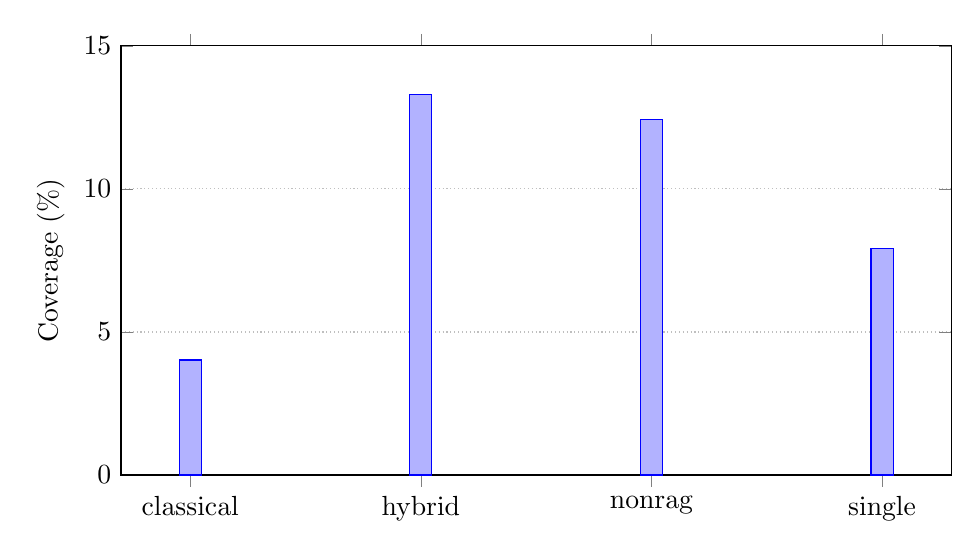
\begin{tikzpicture}
\begin{axis}[
    width=\columnwidth,
    height=0.58\columnwidth,
    ybar,
    bar width=8pt,
    ymin=0,
    ymax=15,
    symbolic x coords={classical,hybrid,nonrag,single},
    xtick=data,
    ylabel={Coverage (\%)},
    ymajorgrids=true,
    grid style=densely dotted
]
\addplot coordinates {(classical,4.02) (hybrid,13.31) (nonrag,12.42) (single,7.93)};
\end{axis}
\end{tikzpicture}
\caption{EduBench completion coverage at freeze time. Hybrid and non-RAG multi-agent are currently processing at more than $3\times$ the observed classical coverage level in this ongoing run.}
\label{fig:edubench_coverage_snapshot}
\end{figure}

\begin{figure}[t]
\centering
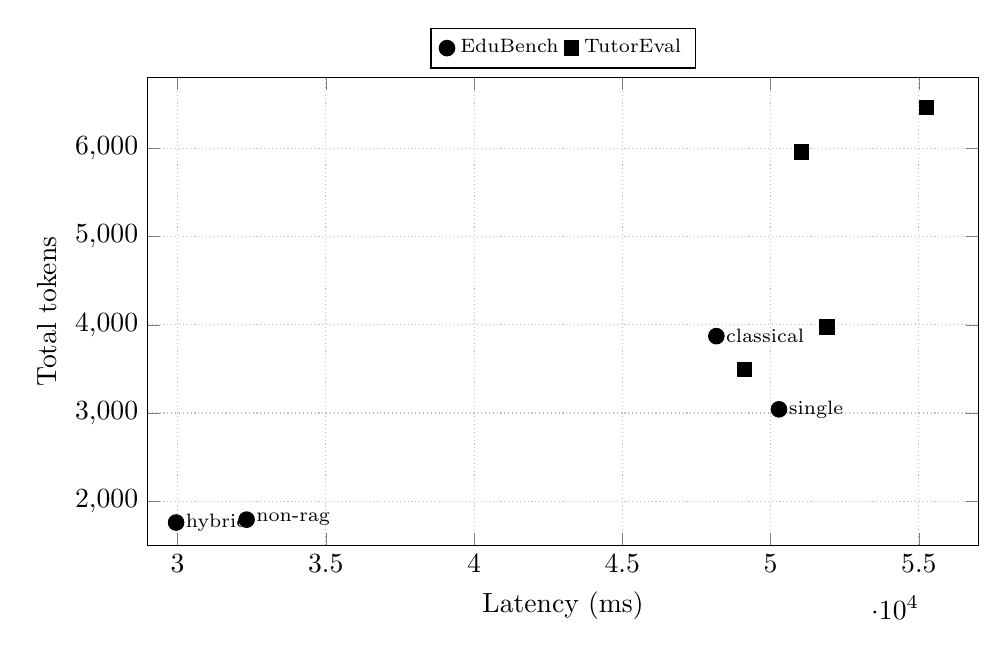
\begin{tikzpicture}
\begin{axis}[
    width=\columnwidth,
    height=0.62\columnwidth,
    xlabel={Latency (ms)},
    ylabel={Total tokens},
    legend style={font=\scriptsize, at={(0.5,1.02)}, anchor=south, legend columns=2},
    xmajorgrids=true,
    ymajorgrids=true,
    grid style=densely dotted,
    xmin=29000,
    xmax=57000,
    ymin=1500,
    ymax=6800
]
\addplot[only marks, mark=*, mark size=2.8pt] coordinates {
    (48170.2,3871.4)
    (29950.7,1757.8)
    (32327.2,1790.7)
    (50282.8,3041.5)
};
\addlegendentry{EduBench}
\addplot[only marks, mark=square*, mark size=2.6pt] coordinates {
    (51903.1,3974.7)
    (49113.4,3490.3)
    (51048.0,5959.3)
    (55257.3,6466.2)
};
\addlegendentry{TutorEval}
\node[font=\scriptsize, anchor=west] at (axis cs:29950.7,1757.8) {hybrid};
\node[font=\scriptsize, anchor=west] at (axis cs:32327.2,1790.7) {non-rag};
\node[font=\scriptsize, anchor=west] at (axis cs:48170.2,3871.4) {classical};
\node[font=\scriptsize, anchor=west] at (axis cs:50282.8,3041.5) {single};
\end{axis}
\end{tikzpicture}
\caption{Latency-token frontier on frozen summaries. Hybrid Fast remains on the most favorable region of the observed quality-efficiency surface across both datasets.}
\label{fig:latency_token_frontier}
\end{figure}

\begin{figure}[t]
\centering
\begin{tikzpicture}[
    node distance=4mm and 6mm,
    every node/.style={font=\scriptsize, align=center},
    box/.style={draw, rounded corners, minimum height=0.9cm, text width=2.4cm, inner sep=2pt},
    decision/.style={draw, diamond, aspect=1.8, inner sep=1pt, text width=1.8cm},
    >={Stealth[length=2mm]}
]
\node[box] (in) {Question + context};
\node[box, below=of in] (fast) {Fast specialists\\planner + diagnoser + rubric};
\node[decision, below=of fast] (u) {$u > \tau$?};
\node[box, below left=6mm and 8mm of u] (keep) {Keep fast path};
\node[box, below right=6mm and 8mm of u] (esc) {Escalate\\retrieve + critic\\or family switch};
\node[box, below=16mm of u] (out) {Tutor output\\with citations};
\node[box, below=of out] (budget) {Budget monitor\\latency, tokens, queries};

\draw[->] (in) -- (fast);
\draw[->] (fast) -- node[right] {uncertainty $u$} (u);
\draw[->] (u) -- node[above left] {no} (keep);
\draw[->] (u) -- node[above right] {yes} (esc);
\draw[->] (keep) |- (out.west);
\draw[->] (esc) |- (out.east);
\draw[->] (out) -- (budget);
\draw[->] (budget.west) .. controls +(-1.2,0) and +(0,-1.0) .. node[left] {budget feedback} (u.south);
\end{tikzpicture}
\caption{Proposed CBRH-2 controller: uncertainty-aware escalation under explicit budget monitoring. The system remains in the cheap specialist path unless expected utility gain justifies additional retrieval or critique cost.}
\label{fig:cbrh2_controller}
\end{figure}
